%    File:    spherical-vs-projected.tex
%    Author:  Marvin Smith
%    Date:    11/7/2015
%


%--------------------------------------------%
%-       Spherical Coordinate Systems       -%
%--------------------------------------------%
\addcontentsline{toc}{subsection}{Spherical Coordinates}
\subsection*{Spherical Coordinates}

Most users are familiar with this first class of coordinates, defined as a \emph{spherical}
coordinate system.  This is commonly referred to the \emph{latitude} and \emph{longitude}.
Spherical coordinates in mathematics typically take the form of $r, \theta,$ and $\phi$ where
$r$ is the radius from the center to the coordinate, $\theta$ is the angle on the x,y plan,
and $\phi$ is the angle from the z axis to xy plane.  Figure \ref{fig:figure_1_2} shows
the relationship between Cartesian and Spherical coordinates. 

\begin{figure}[h!]
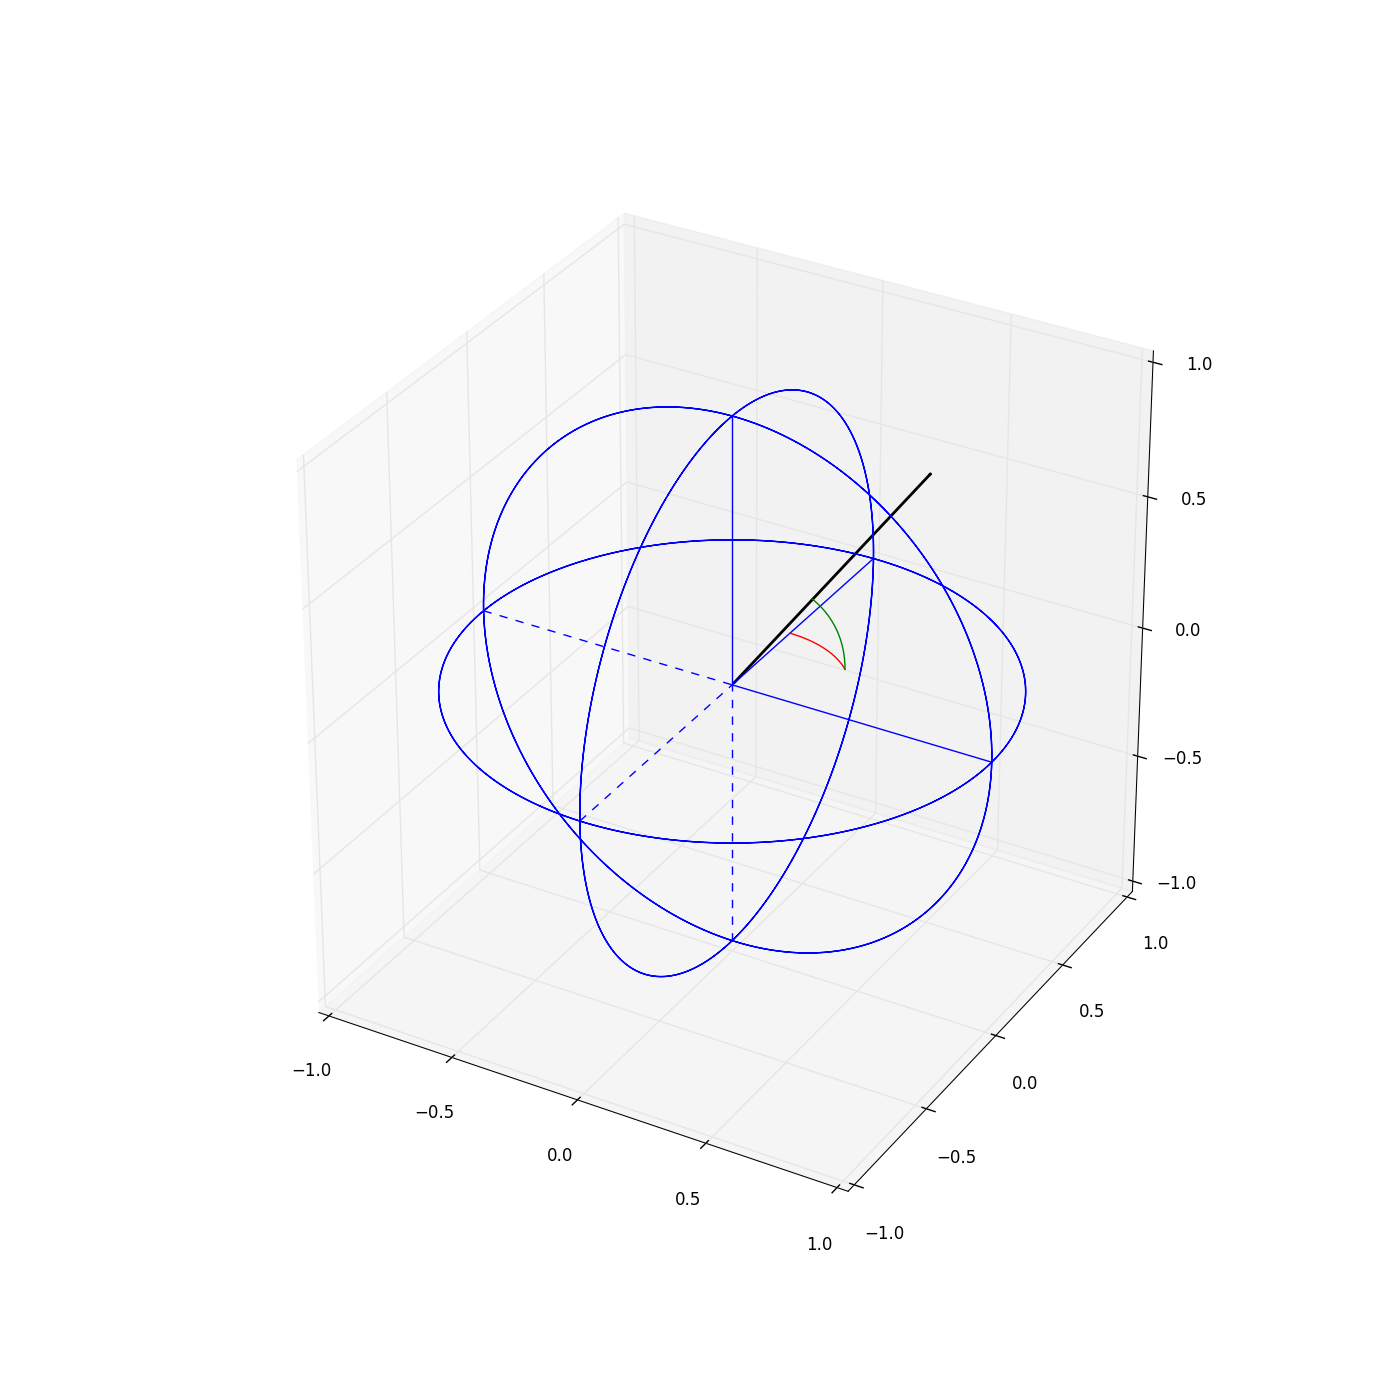
\includegraphics[width=3in]{chapter1/diagrams/figure_1_2.png}
\caption{Relationship between spherical and cartesian coordinates.}
\label{fig:figure_1_2}
\end{figure}

Now to describe spherical coordinates in a Geographic setting, 
$\theta$ becomes \emph{longitude}, $\phi$ becomes \emph{latitude}, and 
$r$ is modified from the distance from the radius, to the distance from the
\emph{datum}.  Datums will be discussed later.  To continue, consider 
a datum as an ellipsoid which models the Earth for which you can describe
the ``sea-level" or zero elevation.  

Geographic coordinates are commonly described in degrees.  Figure 
\ref{fig:figure_1_1} shows the degrees of latitude and longitude
for the Lake Tahoe region of the United States.

\begin{figure}[h!]
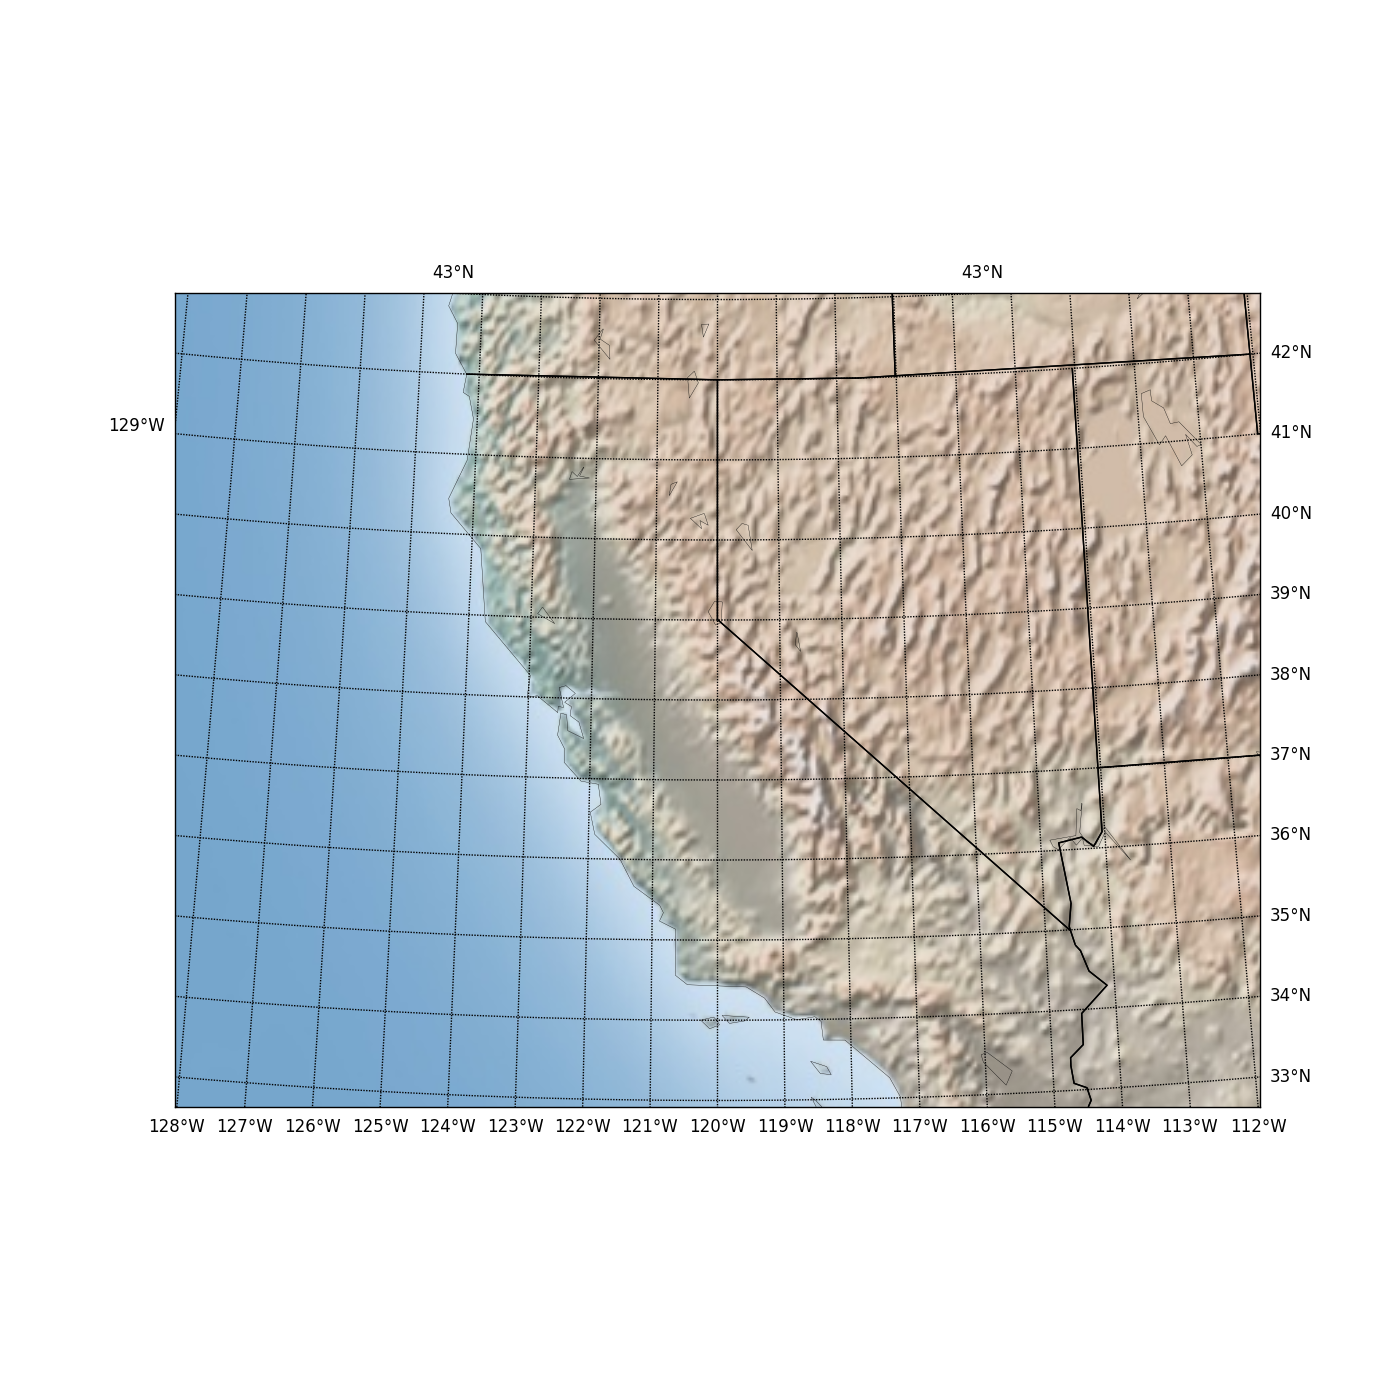
\includegraphics[width=4in]{chapter1/diagrams/figure_1_1.png}
\caption{Shaded relief map of Lake Tahoe showing lines of latitude and longitude.}
\label{fig:figure_1_1}
\end{figure}


\addcontentsline{toc}{subsubsection}{Geographic Coordinate Representation}
\subsubsection*{Geographic Coordinate Representation}

Geographic coordinates in a spherical format can take multiple representations.  The primary focus
here is on the horizontal components, namely the \emph{latitude} and \emph{longitude}.

In this section, we have the coordinate given for Mount Tallac, a mountain near Lake Tahoe in the
Desolation Wilderness.  

\vspace{5mm}
\noindent{\underline{\textbf{Decimal Degrees}}}\\

Decimal Degrees formatting takes the latitude and longitude and represents them as floating-point numbers,
represented in degrees, with a negative number representing the Western and Southern Hemispheres.

\begin{table}[h!]
\begin{tabular}{l l}
\textbf{Latitude} & 38.905984
\end{tabular}
\end{table}

%-------------------------------------------%
%-       Projected Coordinate Systems      -%
%-------------------------------------------%
\addcontentsline{toc}{subsection}{Projected Coordinates}
\subsection*{Projected Coordinates}

Expressing coordinates in latitude and longitude is great for navigation 
as the coordinates are easily relatable to the world-wide coordinates. 
The issue however comes when we try to create maps and other products using
spherical coordinates.  Maps require a 2d \emph{Projection} or \emph{mapping}
from the globe to a flat surface.  


%-----------------------------------------------%
%-        Universal Transverse Mercator        -%
%-----------------------------------------------%
\addcontentsline{toc}{subsubsection}{Universal Transverse Mercator(UTM)}
\subsubsection*{Universal Transverse Mercator (UTM)}

The Universal Transverse Mercator (UTM) is a projected coordinate system based on the
standard \emph{Transverse Mercator} projection.  There are 120 grid zones defined:
60 for Northern and 60 for Southern Hemispheres. 

\begin{figure}[h!]
\centering
\begin{subfigure}[c]{4.2in}
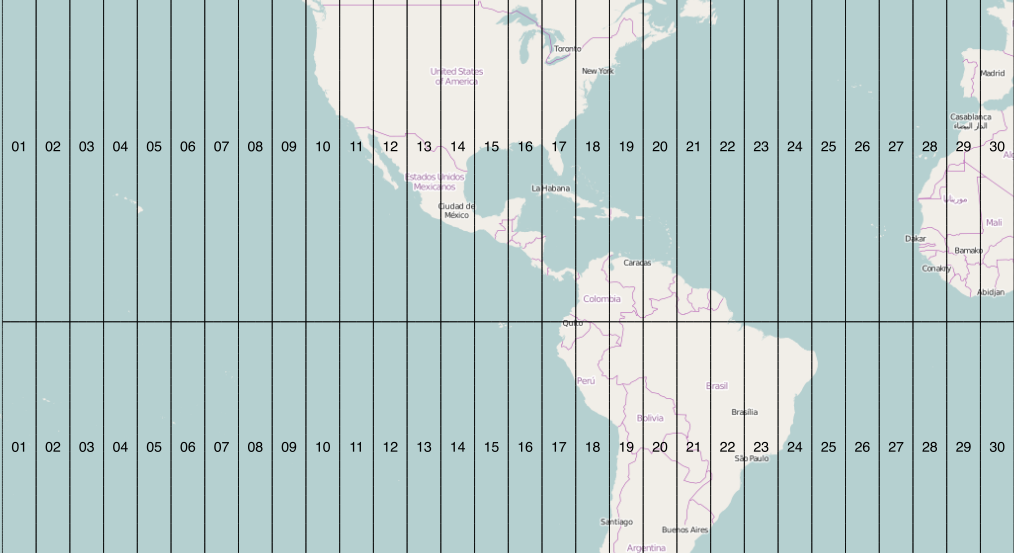
\includegraphics[width=4.2in]{chapter1/diagrams/figure_1_3.png}
\caption{Grid Zones 1-30 N and S}
\end{subfigure}\\
\begin{subfigure}[c]{4.2in}
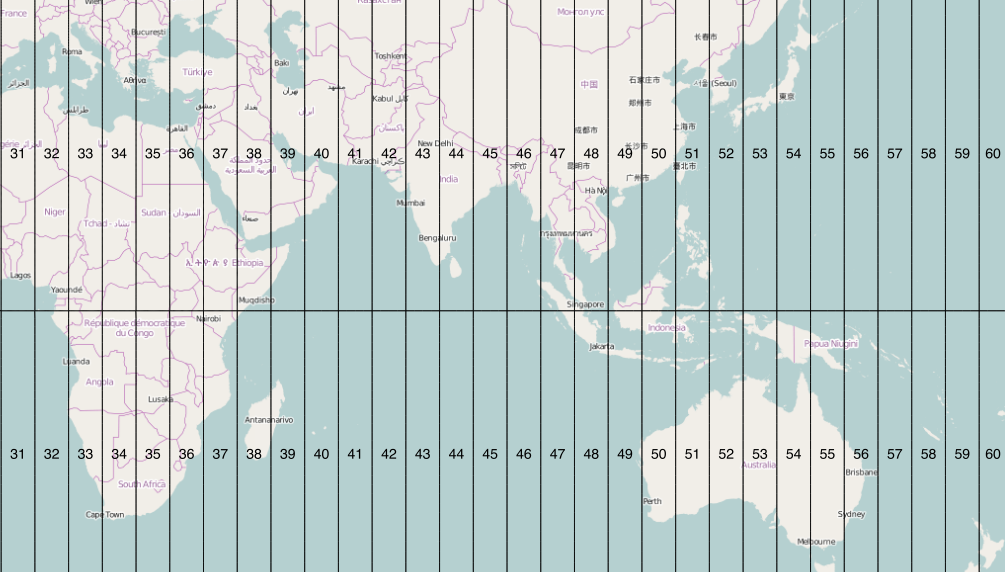
\includegraphics[width=4.2in]{chapter1/diagrams/figure_1_4.png}
\caption{Grid Zones 31-60 N and S}
\end{subfigure}
\caption{UTM Grid Zones. Zones provided by \cite{NGA_SIG_UTM_UPS}, Maps by OSM.}
\end{figure}

Each grid zone has its own parameters defined for the \emph{Centrial Meridian}.
As a consequence, coordinates must be reprojected if moving from one zone to another.

Besides the grid zone, the other components are \emph{easting} and \emph{northing}.
Easting is the $x$ distance from the grid origin and the northing is the $y$-axis
distance from the grid origin.  


%----------------------------------------------%
%-        Universal Polar Stereographic       -%
%----------------------------------------------%
\addcontentsline{toc}{subsubsection}{Universal Polar Stereographic (UPS)}
\subsubsection*{Universal Polar Stereographic (UPS)}





%-----------------------------------------------%
%-       Military Grid Reference System        -%
%-----------------------------------------------%
\addcontentsline{toc}{subsubsection}{Military Grid Reference System (MGRS)}
\subsubsection*{Military Grid Reference System (MGRS)}





%----------------------------------------------%
%-        United States National Grid         -%
%----------------------------------------------%
\addcontentsline{toc}{subsubsection}{United States National Grid (USNG)}
\subsubsection*{United States National Grid (USNG)}

Whereas MGRS is a grid-based projection coordinate system for the entire planet, 
the United States National Grid (USNG) covers only the United States.  USNG 
uses MGRS as the fundamental projection.  In fact, according to \cite[p.~3.1]{USNG_Standard},
MGRS and USNG coordinates are identical.


